
\documentclass[rascunho]{fei}
\usepackage[utf8]{inputenc}
%\usepackage[brazilian]{babel}
\usepackage{verbatim}

\usepackage[caption=false]{subfig}
\usepackage{float}

%\usepackage{subfigure}
%\selectlanguage{brazilian}

\author{Claudio de Oliveira Vilão Junior}
\title{UM SISTEMA DE VISÃO COMPUTACIONAL MONOCULAR PARA UM ROBÔ HUMANOIDE NO DOMÍNIO DO FUTEBOL DE ROBÔS}
%\subtitulo{CONTROLE SERVO-VISUAL DE JOGADORES DE FUTEBOL DE ROBÔS humanoides}
%\cidade{Cidade}
%\instituicao{Instituição de Ensino}

\begin{document}
\overfullrule=2cm
\maketitle

\begin{folhaderosto}
Dissertação de Mestrado apresentada ao Centro Universitário da FEI para obtenção do título de Mestre em Engenharia Elétrica, orientado pelo Prof. Dr. Reinaldo Augusto da Costa Bianchi.
\end{folhaderosto}

%\fichacatalografica
%\folhadeaprovacao
\dedicatoria{As meus pais.}

%\begin{agradecimentos}
%Agradeço ao Latex por não ter vírus.
%\end{agradecimentos}

\epigrafe{A good scientist is a person with original ideas.} {Freeman Dyson}

\begin{resumo}

Onde os algoritmos propostos na literatura não se enquadram no contexto. Apresentar resultados no resumo.


Uma única imagem representa um conjunto de dados de tamanho considerável e tipicamente várias operações precisam ser feitas em cada pixel da referida imagem. Em uma estrutura de vídeo, a qual pode ser assimilado como uma sucessão de várias imagens, esta tarefa torna-se ainda mais difícil, já que, a taxa de quadros por segundo necessita ser mantida. Este trabalho pretende descrever um sistema de visão monocular para quatro robôs humanoides desenvolvidos para participar da liga humanoide na categoria Kid Size, da RoboCup. O sistema de visão proposto permite que os robôs sejam capazes de acompanhar uma bola, identificar os gols, linhas de campo, companheiros e adversários, fornecendo informações, tais como, distâncias e orientações de todos esses objetos simultaneamente, de forma que, todos os processos são executados em tempo real com diferentes resoluções de câmera.

\palavraschave{Robô humanoide, Visão Computacional, Controle Servo-Visual, Rastreamento de objetos, Reconhecimento de objetos }

\end{resumo}

\begin{abstract}

A single image represents a dataset of considerable size, and tipically several operations has to be done in each pixel of that image. In a video structure, which can be assimilated as a succession of several images, this task becomes even more challenging, as the frame rate has to be maintained. This work intends to describe a monocular vision system for four humanoid robots assembled to participate in the Humanoid KidSize League at RoboCup. The proposed vision system allows the robots to be able to track a ball, identify goals, field lines, teammates and  opponents, providing information such as distances and estimated location for the robots simultaneously, via threads. It is possible for all threads to run in real time with different camera resolutions, achieving the main target.

\keywords{Humanoid robot, Computational Vision, Visual servoing, object tracking, object recognition}

\end{abstract}

%\tabelas
%\figuras
%\algoritmos
%\sumario

%Esse foi colocado depois usando o manual.tex
\glsaddall
\listoffigures
\listoftables
\listofalgorithms
%\listoftheorems
\printglossaries
\tableofcontents

%*********************************************************************************************************************************************
%---------------------------------------------------------------------------------------------------------------------------------------------
%---------------------------------------------CAPÍTULO 1 - INTRODUÇÃO ------------------------------------------------------------------------
%---------------------------------------------------------------------------------------------------------------------------------------------
%*********************************************************************************************************************************************
\chapter{Introdução}
\label{chap:introduction}

A Robocup é uma iniciativa educacional de pesquisa, é também uma competição cujo objetivo é incentivar a pesquisa robótica fornecendo desafios nos quais uma grande quantidade de tecnologias possam ser integradas. Jogadores de xadrez artificiais, como o Deep Blue, são bons exemplos do que esse tipo de iniciativa pode fazer pela robótica e a inteligência artificial. 

O conceito de robôs jogadores de futebol foi introduzida em 1993 no Japão, e até hoje, é uma das mais importantes divisões da Robocup. Em 2014, essa competição foi celebrada no Brasil. O objetivo oficial da organização é apresentar, até 2050, um time de robôs jogadores de futebol totalmente autônomos capazes de vencer uma partida, usando as regras oficiais da FIFA, contra a seleção vencedora da Copa do mundo. 

Quatro robôs autônomos (figura ~\ref{Fig:Robos}) foram desenvolvidos pelo time humanoide da FEI para atuar na liga Kid Size da Robocup, de maneira que cada um pudesse apresentar somente características humanas, ou seja, precisavam ter o formato humanoide. O dispositivo de aquisição de imagens precisa estar posicionada na cabeça, além de, necessitar de um processo de decisão e de visão individual livre de controles externos e, é claro, nenhum sensor, a não ser que represente um sentido humano. 



\section{Motivação}

Onde os algoritmos propostos na literatura não se enquadram no contexto. 

A motivação do presente trabalho é desenvolver um sistema de visão computacional robusto e rápido para um robô humanoide, já que um dos maiores problemas da visão computacional, é ter que lidar com a quantidade de informação, muitas vezes irrelevante, e algoritmos que requerem grande esforço de processamento.  





\section{Objetivos}

Este projeto visa desenvolver um sistema servo-visual para um robô humanoide atuante na competição Robocup no ano de 2014, Liga humanoide, categoria Kid Size. Serão desenvolvidos sistemas de visão computacional que permitam ao agente:\\

\begin{enumerate}
	\item Rastrear uma bola, de tamanho conhecido e cor discrepante do fundo, fornecendo sua posição em um sistema de coordenadas;
	\item Identificar linhas de um campo de futebol, assim, como o gol, de modo que essas informações possam ser utilizadas para o agente tomar uma decisão;
	\item Reconhecer agentes do mesmo time e do time rival, possibilitando a realização de passes entre robôs;
	\item Determinar se ele se encontra orientado para o campo de ataque ou de defesa.

\end{enumerate}

\section{Justificativas}
O desenvolvimento de um time de futebol de robôs representa uma aplicação do uso de agentes autônomos com comportamento inteligente, visando a execução de uma tarefa, geralmente complexa, em equipe. O estudo e desenvolvimento da inteligência artificial, fornece desafios e problemas onde diversas tecnologias e metodologias podem ser combinadas para a obtenção dos resultados desejados, especialmente em visão computacional.

\begin{figure}[!t1]
\centering
\includegraphics[width=5.5in]{Imagens/robos.jpg}
\DeclareGraphicsExtensions.
\caption{Robôs desenvolvidos.\\ Fonte: o Autor}
\label{Fig:Robos}
\end{figure}

\section{Histórico}

A primeira edição da Robocup aconteceu em 1997 em Nagoya, no Japão, depois de se ter organizado uma pré-Robocup em Osaka, no mesmo país, com finalidades de encontrar possíveis dificuldades e problemas na organização desse tipo evento em escala global. A iniciativa foi lançada pelo Dr. Hiroaki Kitano (Tóquio), um pesquisador na área de Inteligência Artificial que se tornou presidente e fundador da Robocup Federation.


\begin{table}[ht!]
    \caption{Histórico Robocup} 
    \centering
    \begin{tabular}{|c|c|c|c|}
    \hline 
    Competição & Ano & Cidade & País Sede \\ 
    \hline 
    Robocup & 2015 & Hefei & China \\ 
    \hline 
    Robocup & 2014 & João Pessoa & Brasil \\ 
    \hline 
    Robocup & 2013 & Eindhoven & Holanda \\ 
    \hline 
    Robocup & 2012 & Cidade do México & México \\ 
    \hline 
    Robocup & 2011 & Istambul & Turquia \\ 
    \hline 
    Robocup & 2010 & * & Singapura \\ 
    \hline 
    Robocup & 2009 & Graz & Áustria \\ 
    \hline 
    Robocup & 2008 & Suzhou & China \\ 
    \hline 
    Robocup & 2007 & Atlanta & Estados Unidos \\ 
    \hline 
    Robocup & 2006 & Bremen & Alemanha \\ 
    \hline 
    Robocup & 2005 & Osaka & Japão \\ 
    \hline 
    Robocup & 2004 & Lisboa & Portugal \\ 
    \hline 
    Robocup & 2003 & Pádova & Itália \\ 
    \hline 
    Robocup & 2002 & Fukuoka/Busan & Japão/ Coréia do Sul \\ 
    \hline 
    Robocup & 2001 & Seatle & Estados Unidos \\ 
    \hline 
    Robocup & 2000 & Melbourne & Austrália \\ 
    \hline 
    Robocup & 1999 & Estocolmo & Suécia \\ 
    \hline 
    Robocup & 1998 & Paris & França \\ 
    \hline 
    Robocup & 1997 & Nagoya & Japão \\ 
    \hline 
    \end{tabular}
	\label{tbl:historico}
    \caption*{Fonte: \citeonline{Rules}}
\end{table}

\section{Domínio}

O projeto tem como base a principal competição de futebol para robôs, a Robocup, sendo a liga de atuação do agente a Humanoid League na categoria Kid Size. Todos os dados dessa seção estão de acordo com o livro de regras de 2014 da Robocup.

O campo de jogo consiste de uma superfície plana e nivelada, coberta por um carpete verde. As linhas brancas têm 5 centímetros de largura. Segmentos de linha de 10 centímetros de largura são usados para a marca de penalty e a posição inicial do início da partida. O campo é limitado pelas linha maiores, chamadas laterais, e por linhas menores, definidas como sendo de fundo, onde se encontram os gols. Todas as áreas localizadas fora dessas quatro linhas são consideradas desconhecidas e indefinidas. Os gols são compostos por duas traves, um travessão e uma rede. O travessão, bem como as traves dos gols são amarelos, o trançado da malha da rede não possui aberturas maiores do que 4 centímetros e sua cor poderá ser cinza ou preta. 

São utilizadas apenas lâmpadas como forma de iluminação. Porém, as condições de iluminação dependem do local da competição. O campo é iluminado de forma constante e com brilho suficiente, sem influência da luz do dia. Em volta do campo, um local é definido onde somente o juiz, seus assistentes e mais dois manipuladores dos robôs podem atuar. Nenhum participante pode usar, abaixo da cintura, cores iguais ou similares às definidas para o campo, bola ou gols. Em 2014, a bola possuía coloração laranja, dois times jogavam por vez e cada time de futebol poderia ter no máximo quatro jogadores. 

Apenas os sensores equivalentes aos sentidos humanos são permitidos, mas, não são obrigatórios. Robôs humanoides devem ter o formato de seus corpos semelhante ao do ser humano, devem ter pernas e braços. Uma série de restrições são aplicadas às medidas dos agentes, uma delas, que tem mais relevância para a pesquisa, é a relação entre a altura do corpo do robô \(H_{\text{Robô}}\) e a altura da cabeça \(H_{\text{Cabeça}}\), como segue:

A altura da cabeça, incluindo o pescoço, deve satisfazer a seguinte expressão:\hfill 

%\hspace{80}
\begin{equation}
0,05 * H_{\text{Robô}} \leq H_{\text{Cabeça}} \leq 0,25 * H_{\text{Robô}}  \\
\end{equation}
Onde a altura da cabeça é definida, como sendo, a distância do eixo da primeira junta do braço, no ombro, até o topo da cabeça.

\begin{table}[ht!]
    \caption{Medidas Importantes do Campo, da Bola e dos Jogadores} \label{tbl:medidas}
    \centering
    \begin{tabular}{|c|c|c|c|}
    \hline 
    Descrição & Comprimento (cm) \\ 
    \hline 
    Linha Lateral ( Comprimento do Campo) & 900  \\ 
    \hline 
    Linha de Fundo ( Largura do Campo) & 600 \\ 
    \hline 
    Largura da grande área & 60 \\ 
    \hline 
    Comprimento da grande área & 345 \\ 
    \hline 
    Diâmetro do grande círculo & 150 \\ 
    \hline 
    Diâmetro da Bola & 10 \\ 
    \hline 
    Altura Máxima dos Agentes & 90 \\ 
    \hline 
    Largura dos Gols & 225 \\ 
    \hline
    Altura dos Gols & 110 \\
    \hline
    Altura das malhas dos Gols & 100 \\
    \hline
    Largura das traves e travessões & 10 \\
    \hline


    \end{tabular}
    \caption*{Fonte: Livro de Regras Robocup - (Robocup Rules Book), 2014 \cite{Rules}}
\end{table}

O campo de visão dos robôs é limitado a 180 graus, isso significa que o ângulo máximo entre quaisquer dois pontos na sobreposição do campo de visão, de todas as câmeras montadas sobre o robô, precisam ser inferiores a esse ângulo. 

O mecanismo para girar (pan) a câmera é limitado a 270 graus, 135 graus para cada lado, contados da posição de olhar para frente. Já o mecanismo para erguer (tilt) a câmera é limitado a 90 graus medidos da linha horizontal, essas restrições simulam as mesmas limitações das juntas do pescoço humano. 

Seguindo essa linha de limitações humanas, fica definido que, de qualquer posição do robô, de qualquer ângulo de câmera ou do robô, o mesmo não pode ser capaz de visualizar os dois gols ao mesmo tempo, e o número de câmeras fica limitado a duas, porém, a visão monocular também é permitida, de qualquer forma deve(m) estar na cabeça do robô.

Robôs participantes das competições da liga humanoide devem ser, predominantemente, pretos, cinzas, prateados ou brancos, com as limitações de serem não reflexivos e terem o pés pretos. Qualquer cor do campo, gol, bola ou time adversário deve ser evitada no robô. Braços, pernas e corpos devem ter aparência sólida e devem estar marcadas com a cor magenta (para agentes do time vermelho) e com a cor ciano (para agentes do time azul), ambas as marcas devem ter no mínimo 5 centímetros e estar visíveis nos dois lados das pernas e braços.

\section{Organização do Trabalho}

As seções anteriores apresentaram domínio, justificativas, objetivos, histórico e motivação deste trabalho, compondo o capítulo introdutório. Os demais capítulos estão estruturados da seguinte maneira:

Conceitos básicos de aquisição, processamento e representação de imagens digitais são abordados no capítulo 2, apresentando, em forma de revisão, alguns dos mais conceituados algoritmos de processamento digital de imagens contextualizando-os com a visão computacional, a pesquisa prossegue com o capítulo 3, em que trabalhos correlatos são estudados e é posto em perspectiva o modo como algumas equipes participantes da Robocup utilizam algoritmos de processamento digital de imagens na forma de visão computacional, de maneira que, é possível visualizar como solucionaram os mais variados problemas visuais do jogo de futebol.

A visão do agente foi baseada no que outras equipes têm feito, mas, também, em conceituados algoritmos de visão computacional. A descrição desse sistema de visão, com fluxogramas e testes a serem feitos, é apresentada na proposta de trabalho abarcada pelo capítulo 4. O capítulo 5 traz os testes já executados, os quais geraram alguns resultados preliminares. Por fim, nas Considerações Finais, no capítulo 6, é feita uma breve síntese das atividades realizadas até o momento, apontado para perspectivas futuras, por meio de um Cronograma de atividades.


%%===============================================================================


%*********************************************************************************************************************************************
%---------------------------------------------------------------------------------------------------------------------------------------------
%---------------------------------------------CAPÍTULO 2 - FUNDAMENTAÇÃO TEÓRICA--------------------------------------------------------------
%---------------------------------------------------------------------------------------------------------------------------------------------
%*********************************************************************************************************************************************

\chapter{Fundamentação Teórica: Visão Computacional}
\label{chap:revision}
\input{revision}

\section{Processamento de imagens coloridas}
A interpretação de cores feita pelo ser humano é um fenômeno fisiopsicológico, compreendido apenas em partes, porém podemos definir formalmente a natureza da cor experimentalmente e teoricamente. A cor é uma das características mais largamente utilizadas em diversos sistemas por ser relativamente independente quanto ao tamanho, orientação e resolução da imagem e é computacionalmente menos cara quando comparada aos demais descritores \cite{Bender}. 

Para entender como os descritores de cor são utilizados, é necessário definir previamente o conceito de cor e listar algumas de suas características. A cor pode ser definida como um fenômeno perceptual da luz quando incide e é refletida por um objeto. Como se pode observar, o conceito de cor é diretamente relacionado ao conceito de luz \cite {Gonzalez}. Portanto, ao se referir ao conceito de cor deve-se mencionar, obrigatoriamente, a luz.

Da interação entre a energia luminosa e o meio, a cor pode se formar através de (a) processo aditivo, (b) processo subtrativo e (c) formação por pigmentação \cite{Bender}. No processo aditivo ocorre a combinação entre raios de luz com frequências diferentes através da soma de energia dos fótons. No processo de formação subtrativo, a luz é transmitida através de um filtro que absorve a radiação luminosa de um determinado comprimento de onda. Alternativamente, a luz também pode incidir através de um corante, que é constituído por filtros que podem absorver a radiação luminosa de um determinado comprimento de onda. Finalmente, no processo de formação por pigmentação, os pigmentos podem absorver, refletir ou transmitir a radiação luminosa. 

Dois conceitos preliminares são particularmente importantes para o entendimento do conceito de percepção de cor. São eles: a luminância e a crominância. A luminância contém a informação da quantidade das cores pretas e brancas presentes em uma imagem. O cérebro humano interpreta essa informação como a quantidade de cinza presente na cor (ou brilho). A crominância informa a respeito da tonalidade de uma cor. É a frequência dominante do raio de luz. A combinação destes dois conceitos, em diferentes proporções, permite ao cérebro perceber o espectro de cores visível em uma determinada imagem ou cena. Para representar as cores existem modelos ou sistemas de cores \cite {Gonzalez}, como por exemplo RGB (“red, green, blue”), CMY (“cyan, magenta, yellow”),HSI (“matiz, saturação, intensidade”), YIQ (luminância, em-fase, quadratura) e LAB (luminosidade, verde-vermelho, azul-amarelo).

O sistema Red, Green, Blue é um sistema de representação de cor \cite{Bimbo} aditivo e se baseia na teoria dos três estímulos proposta por \cite{Young}. Segundo essa teoria, o olho humano percebe a cor através do estímulo de três pigmentos visuais presentes nos cones da retina, que possuem sensibilidades para alguns comprimentos de onda, como por exemplo, 630 nanômetros (vermelho – red), 530 nanômetros (verde – green) e 450 nanômetros (azul – blue). Uma representação desse sistema pode ser formulada através de um cubo com os eixos R, G e B. Podemos dizer que a origem representa a cor preta, os vértices das coordenadas (1, 1, 1) representam o branco, os vértices que estão sobre os eixos representam as cores primárias e os vértices restantes representam os complementos das primárias. 

É importante observar que cada ponto no interior do cubo corresponde a uma cor, representada por uma tripla (R, G, B), com os valores de R, G e B variando de 0 a 1. Os tons de cinza são representados ao longo da diagonal principal do cubo, que se inicia no ponto de origem até o vértice que foi apontado como a cor branca. Portanto, é possível, afirmar que cada tom de cinza presente no cubo é formado por contribuições iguais das cores primárias que o compõem. Um exemplo de tom de cinza médio poderia ser representado pela tripla (0.5, 0.5, 0.5).



\section{Filtros}
\input{filters}

\section{Médio Nível - Regionalização de Partes das Imagens}
\subsection{Segmentação}

A segmentação, em visão computacional, é o processo de dividir ou segregar uma imagem digital em duas ou mais regiões diferentes, com o objetivo de simplificar de uma imagem visando facilitar a sua análise ou interpretação. Os retornos esperados, como resultados do processo de segmentação, são atributos dessa imagem, como, regiões e contornos. Convém elucidar a diferença entre borda e contorno, a borda se verifica como sendo uma transição de uma parte do contorno de um objeto. A maior dificuldade é interpretar quais bordas pertencem, efetivamente, ao contorno de uma região ou objeto.

Cada um dos pixels em uma mesma região é segmentada, levando-se em consideração alguma característica ou propriedade computacional. São propriedades comuns a cor, a intensidade, a textura ou, mesmo, a continuidade. 

Todas as regiões selecionadas devem possuir limiares de características que permitam sua discretização umas das outras. De acordo com \citeonline{Benallal} e \citeonline{Broggi} é possível efetuar a segmentação seguida de reconhecimento de formato em tempo real. 

\begin{figure}[!h1]
\centering
\includegraphics[width=2.5in]{Imagens/Seg_Hsv.png}
\includegraphics[width=2.5in]{Imagens/Seg.jpeg}
\DeclareGraphicsExtensions.
\caption{Segmentação do Laranja usando como entrada uma imagem no modelo de cores HSI. \\ Fonte: o Autor}
\label{Fig:Seg}
\end{figure}


\subsection{Morfologia Matemática}

Morfologia é o estudo da forma, sendo o estudo morfológico o estudo das estruturas dessa forma. Em linguística, morfologia é o estudo da estrutura das palavras. Em biologia, morfologia está mais diretamente relacionada à forma de um organismo, por exemplo, a forma de uma folha pode ser usada para identificar uma planta ou a forma de uma colônia de bactérias pode ser usada para identificar sua variedade.
Por outro lado, os matemáticos consideram a morfologia uma parte da teoria de conjuntos, e por consequência, denomina-se morfologia matemática como sendo um conjunto de métodos, inicialmente desenvolvidos por \citeonline{Matheron}, que tem em comum o objetivo de estudar a estrutura geométrica de um objeto ou parte dele. 

Segundo \citeonline{Dougherty}, é possível definir a morfologia digital como sendo um caminho para descrever ou analisar a forma de um objeto digital, levando-se em conta sua estrutura geométrica, baseado no fato de que uma imagem consiste em um conjunto de pixels, que podem ser reunidos em grupos, criando uma estrutura bidimensional (forma). Nesse estudo fica subentendida a referência à morfologia digital. Certas operações matemáticas, quando aplicadas em conjuntos de pixels, podem ser usadas para ressaltar aspectos específicos das formas permitindo que sejam contadas ou reconhecidas.

A base da morfologia segundo \citeonline{Gonzalez} consiste em extrair as informações relativas à geometria e à topologia de um conjunto desconhecido (no caso uma imagem) pela transformação através de outro conjunto bem definido, chamado elemento estruturante. Operações morfológicas estão divididas em binárias (aplicadas a imagens com pixels pretos ou brancos), e sobre imagens coloridas (aplicadas a imagens em tons de cinza ou, como o próprio nome diz, em imagens coloridas).

Após processamento, um objeto é considerado um conjunto matemático de pixels brancos, sendo, cada pixel, identificado pelos seus índices de linha e coluna. No caso de operações binárias, um pixel afetado por essa operação será substituído pelo seu valor oposto. Em operações executadas em imagens coloridas pode ocorrer apenas a modificação parcial do valor do pixel.
Com isso torna importante ao contexto a utilização de teoria dos conjuntos, pois é a base utilizada na morfologia, assim, é com esta teoria que será descrita e apresentada uma imagem.  

\begin{figure}[!ht1]
\centering
\includegraphics[width=2.5in]{Imagens/Morphology.jpeg}
\DeclareGraphicsExtensions.
\caption{Exemplo de erosão e dilatação para um objeto circular, com elemento estruturante circular. \\ Fonte: o Autor}
\label{Fig:Morfologia}
\end{figure}

As operações básicas da morfologia digital são a erosão, em que pixels que não atendem a um dado padrão são apagados da imagem, e a dilatação, em que uma pequena área relacionada a um pixel é alterada para um dado padrão. Todavia, dependendo do tipo de imagem que está sendo processada (preto e banco, tons de cinza ou colorida), a definição dessas operações muda, assim, cada tipo deve ser considerado separadamente.



\subsection{Transformada de Hough}

Sendo uma ferramenta de uso comum em visão computacional, a transformada de \\Hough é um processo matemático que detecta formas geométricas em imagens digitais. Essa técnica, desenvolvida por \citeonline{Hough}, encontra formas que são paramatrizáveis em imagens digitais como linhas, círculos e elipses, mesmo em imagens com pouca visibilidade da forma ou imagens fortemente ruidosas.

Em geral, a transformada é aplicada após a imagem sofrer um pré-processamento, comumente a detecção de bordas.A transformada de Hough encontra uma relação entre o espaço de imagem e o espaço de parâmetros. Cada transição (ou borda) de uma imagem é transformada por um mapeamento para determinar sua relação no espaço de parâmetros através de um vetor. 

As posições do vetor são incrementadas e indicarão quais os parâmetros correspondentes à forma especificada, através do máximo local do acumulador. A detecção de retas foi sua primeira aplicação mas, a transformada de Hough foi modificada para possibilitar a localização de outras formas geométricas. A transformada de Hough utilizada, majoritariamente, atualmente pode ser atribuída a \citeonline{HoughCircle} e a \citeonline{FastHough}.

Hough usou a equação definida por y = a.x + b como representação paramétrica de uma linha, fato que conduziu a soluções infinitas para linhas paralelas ao eixo y, cuja solução será abordada posteriormente.
 
O algoritmo de Hough requer um acumulador de dimensão igual ao número de parâmetros desconhecidos. Por exemplo: achar segmentos de linhas usando a equação y = ax + b, requer achar dois parâmetros para cada segmento: a e b, ou seja, duas dimensões da matriz acumuladora.

Assim, usando uma matriz acumuladora A, o procedimento de Hough examina cada pixel e calcula os parâmetros da curva (equação) especificada que passa pelo pixel. 
O procedimento examina cada pixel e calcula os parâmetros da equação de reta que passa por esse pixel, incrementando a matriz acumuladora.

Caso uma imagem que não foi pré-processada com algoritmo de detecção de bordas, fato incomum na transformada de Hough, será examinado o pixel e sua vizinhança na imagem para determinar se há evidência de borda ou transição naquele pixel. Quando todos pixels tiverem sido processados, procura-se na matriz acumuladora os maiores valores. Esses valores indicam os parâmetros de prováveis linhas na imagem.

Ao procurar os máximos na matriz acumuladora, lança-se o artifício do uso de um limiar, visando encontrar uma quantidade mínima de pontos colineares. Qualquer valor da matriz acumuladora que não for superior ao limiar será ignorado. As detecções de outras formas, utilizando a transformada de Hough, usam o mesmo princípio, com a ressalva na quantidade de parâmetros da equação que será empregada, e em consequência na dimensão do acumulador.
 
\citeonline{HoughCircle} sugeriram coordenadas polares para representação de uma linha. Essa modificação manteve a quantidade de dimensões da matriz acumuladora e resolveu a limitação inicial de linhas paralelas ao eixo y. Usando esta parametrização, todo o ponto (x,y) na equação da reta satisfará a equação r= x . cos ( q ) + y . sin ( q ). Onde os parâmetros r e q são respectivamente a distância e a orientação da linha normal à reta candidata.

Cada pixel do espaço da imagem produz uma função senoidal no espaço de Hough que alimenta um histograma. Com muitas senóides, ou seja, muitas possíveis linhas, o histograma gera diversos máximos que não correspondem efetivamente às linhas. Para resolver essa dificuldade, encontra-se a maior linha da imagem e remove-se sua contribuição do histograma. Repetindo esse procedimento até o fim das linhas encontradas, encontra-se o máximo global.

Como uma forma de inferir um formato circular à bola, é usada a transformada de Hough para círculos, na implementação sugerida por \citeonline{Davies}. Essas formas são parametrizados por "x", "y" e "r", onde "x" e "y" referem-se a posição de centro e "r" ao raio do círculo. Agora que a matriz acumuladora têm três dimensões, é necessário reduzir a complexidade computacional da transformada de Hough. Determinar o centro e em seguida, encontrar o raio divide o problema em duas fases distintas, amenizando as dificuldades computacionais dessa técnica.

Fica definido que a normal tangente de qualquer pixel pertencente a um círculo passa pelo centro desse círculo. Calcula-se a tangente como a linha que se ajusta melhor a todos pixels de uma vizinhança pequena (usando o método mínimos-quadrado), isso permite calcular a normal e registrá-la em um histograma. Finalmente, os máximos do histograma definem os locais de centros dos possíveis círculos. 

Encontrar o raio esconde uma dificuldade prática, existem infinitos círculos que podem ter o mesmo centro. Para sobrepor essa dificuldade, alimenta-se um histograma unidimensional com a distância de cada pixel até o centro de um determinado círculo. Assim, os máximos dos histogramas correspondem aos raios dos círculos.

Há ainda, a transformada probabilística de Hough, que afirma que é suficiente computar a transformada de Hough só de uma proporção de pixels na imagem. Estes pixels são escolhidos de forma aleatória usando-se uma função de densidade de probabilidade uniforme. Essa técnica foi  proposta por \citeonline{Kiryatti}.


\subsection{Condensação}

O algoritmo de condensação (Propagação densidade condicional) é um algoritmo de visão computacional. Sua aplicação principal é detectar e rastrear objetos que se movem em um ambiente desordenado. Ser capaz de identificar quais os pixels de uma imagem compõem um objeto é um problema não-trivial. A condensação é um algoritmo probabilístico que tenta resolver este problema.

O próprio algoritmo é descrito em detalhe por Isard e Blake numa publicação no International Journal of Computer Vision em 1998. [1] Um dos aspectos mais interessantes do algoritmo é que ele não é calculado em cada pixel da imagem. Em vez disso, os pixels são escolhidos ao acaso, e apenas um subconjunto dos pixels acaba sendo processado. A presença de desordem tende a produzir distribuições de probabilidades para o estado do objeto que são multi-modais e, portanto, poderiam ser mal modelados pelo filtro de Kalman.





\begin{comment}

\subsection{Momentos}

Momentos são utilizados para extração de características de uma imagem. A partir de uma imagem segmentada é possível descrever a distribuição espacial dos pontos contidos na imagem ou em uma região. Será feita uma pequena introdução de como calcular baricentros de figuras planas para definir os momentos de uma imagem digital, visando facilitar o entendimento do conceito.

Se toda massa de um corpo estiver concentrada sobre um ponto, a esse ponto é dado o nome de baricentro ou centroide. Seguindo essa linha, o seu cálculo depende da distribuição da massa do corpo. Se os pontos desse objeto estiverem distribuídos de uma forma não homogênea, o centro de massa pode não se encontrar dentro do corpo

O centro de massa de duas partículas (pontuais) localizadas em \(P_1 e P_2\) , com massas \(m_1\) e \(m_2\) é um ponto C no segmento de reta que une \(P_1\) a \(P_2\) a uma distância ponderada pelos valores \(m_1\) e \(m_2\). A ponderação é feita da seguinte maneira: a distância de \(P_1\) a C está para a distância de \(P_1\) a \(P_2\), assim como, a massa \(m_2\) está para a massa total \(m_1 + m_2\). Isto é:

\begin{equation}
\frac{ \bar{P_1C} } { \bar{P_1 P_2} } = \frac{ m_1 } { m_1 + m_2}
\end{equation}

Em imagens digitais os pontos são pixels e o equivalente à sua massa é estimada por sua intensidade ou área ocupada por esses pixels. Momentos de imagens são úteis para descrever objetos após segmentação. Propriedades simples da imagem, que são encontradas via momentos, incluem área ou intensidade total, centroide e informação sobre sua orientação. A primeira menção ao termo momentos em imagens digitais vem de \citeonline{Hu}.


\subsection{Momentos centrais}

A partir dos momentos é possível definir, segundo \citeonline{Flusser} algumas medidas importantes sobre os objetos de interesse, e que são úteis na identificação de diferentes formas, por exemplo, os momentos regulares de ordem 0 e 1 são usados para o cálculo do baricentro ou centro de massa do objeto. Momentos centrais são definidos da seguinte forma:

\begin{equation}
\displaystyle \mu_p{}_q = \int_{-\infty}^{\infty}\int_{-\infty}^{\infty}(x - \bar{x})^p . (y - \bar{y})^q f(x,y) dx dy
\end{equation}\\

Nessa fórmula $(\mu_{pq})$ é o momento de ordem (p+q) da função intensidades e os limites da integral representam respectivamente a largura e a altura da imagem digital. 

\subsection{Momentos de Primeira Ordem}

O momento de uma área plana em relação a um eixo é o produto de sua área pela distância de seu centroide ao referido eixo. O momento de uma região digital é calculada, computando-se a distância de cada pixel num processo equivalente ao de cálculo de centro de massa em um objeto bi-dimensional.  

O teorema de Green \cite{Green} relaciona a integral de linha ao longo de uma curva fechada no plano com a integral dupla sobre a região limitada por essa curva, em outras palavras, é possível determinar a área de figuras planas somente integrando pelo perímetro desses objetos.

O momento de uma imagem é uma média ponderada das intensidades dos pixels de uma imagem.

\begin{equation}
 mu_i{}_j = \sum\limits_{x,y} [ Array(x,y) . (x - \bar{x})^j . (y - \bar{y})^i ]
\end{equation}\\

onde $(\bar{x}, \bar{y})$ , é o centro de massa do objeto digital.

\begin{equation}
\bar{x} = \frac{m_1{}_0}{m_0{}_0} \textrm{ , }  \bar{y} = \frac{m_0{}_1}{m_0{}_0}
\end{equation}\\

Os momentos centrais normalizados, ou seja, invariantes à rotação e escala, são calculados da seguinte forma:

\begin{equation}
 nu_i{}_j = \frac{mu_i{}_j} { m_0{}_0 ^\frac{i+j}{2+1} }
\end{equation}\\

A informação sobre a orientação da imagem pode ser derivada  usando os momentos centrais de primeira ordem para construir uma matriz de covariância. Os autovetores dessa matriz correspondem aos eixos de maior e menor intensidade, dessa forma é possível extrair a orientação do objeto digital. Extraindo o autovetor com maior valor e, assim, definindo sua elongacionalidade.

Definindo todas as possíveis posições do centro de massa dentro do objeto, tem-se a envoltória convexa ou fecho convexo do objeto. De outra forma ele é o “menor” conjunto convexo que contém esses pontos

\end{comment}









\section{Alto Nível}
	\subsection{Máquina de Vetores de Suporte - SVM}
	\input{svm}

	\subsection{Adaboost}
	\input{adaboost}

\section{Controle Servo-Visual}
O controle servo-visual é uma técnica que usa o retorno de dados extraídos de um sensor de visão para controlar o movimento do robô. Esse tipo de controle, para o domínio sugerido, se restringe ao controle dos dois servo-mecanismos referentes à cabeça do robô, mais especificamente do pescoço.

Uma das primeiras abordagens referentes ao controle servo-visual foi publicado por \citeonline{Corke}.Trabalhos mais recentes foram publicados por \citeonline{VS1} e por \citeonline{VS2}, aqui de uma forma mais abrangente no qual entende-se por controle servo-visual todas as ações feitas pelo robô que possuem como origem a visão do mesmo, inclusive movimentos das mãos, pés, rodas e articulações.

Técnicas de controle servo visual são classificados nos seguintes tipos:
\begin{enumerate}
     \item Baseada em Imagem (IBVS)
     \item Baseado Posição / Pose  (PBVS)
     \item Abordagem Híbrida
\end{enumerate}

A IBVS foi proposta por \citeonline{Weiss}. A lei de controle é baseada no erro entre as características atuais e desejadas no plano da imagem e não envolve qualquer estimativa da pose do alvo. Os recursos podem ser as coordenadas de recursos visuais, linhas ou momentos de regiões. A IBVS tem dificuldade com movimentos muito grandes, como rotações, o que veio a ser chamado retiro de câmera. \footnote{Do inglês: "Camera Retreat"}

A PBVS é uma técnica baseada em uma única câmera. Isto porque a posição do objeto de interesse é estimada em relação à câmera e, em seguida, é emitido um comando para o controlador de robô, que por sua vez, controla o robô. Neste caso, as características da imagem são extraídas mas, são, também, utilizadas para estimar a pose do objeto no espaço cartesiano.

Abordagens híbridas usam uma combinação dos controles previamente descritos. De forma geral, essas duas técnicas são consideradas passivas já que aguardam os dados do sensor de visão para tomar alguma decisão. 

Uma outra forma de encarar esse desafio é usar uma visão ativa, como proposta por \citeonline{Sharma}, que, de fato, procura ativamente o objeto a ser identificado e para tanto precisa tomar algumas decisões, mesmo que não haja dados relevantes vindos da câmera. 

Um sistema de visão ativo é capaz de interagir com o seu meio ambiente, alterando o seu ponto de vista em vez de observá-lo passivamente e operando em sequências de imagens, em vez de em um único quadro. Além disso, a capacidade de acompanhar fisicamente um alvo reduz o borrão de movimento, aumentando a resolução de destino para tarefas de nível mais elevado, tais como classificação. 

O controle servo-visual armazena as posições de trajetória do objeto e, por meio de regressão, estima as próximas posições do mesmo.  	Usando um algoritmo guloso encontra-se o melhor movimento antecipado da câmera em direção ao objeto. Para garantir um movimento plausível da câmera, é necessário considerar a cinemática e a dinâmica desse movimento, otimizando a trajetória da câmera para que essa possa manter o objeto em seu campo de visão.

Uma das vertentes da visão ativa é a configuração escravo-mestre \cite[p.2]{Fernandez}, no qual uma câmera está fixa e outra está em movimento. Ambas precisam estar em um mesmo sistema de coordenadas para que as informações trocadas entre elas sejam facilmente interpretadas. Essa configuração poderá ser usada em um projeto futuro, no qual o goleiro exerça o papel de câmera estática de supervisão enquanto os outros jogadores seriam as câmeras ativas em movimento. 




%*********************************************************************************************************************************************
%---------------------------------------------------------------------------------------------------------------------------------------------
%---------------------------------------------CAPÍTULO 3 - TRABALHO CORRELATOS----------------------------------------------------------------
%---------------------------------------------------------------------------------------------------------------------------------------------
%*********************************************************************************************************************************************

\chapter{Trabalhos Correlatos}
\label{chap:relatedwork}
\input{relatedwork}

%*********************************************************************************************************************************************
%---------------------------------------------------------------------------------------------------------------------------------------------
%-------------------------------------------  CAPÍTULO 4 - PROPOSTA --------------------------------------------------------------------------
%---------------------------------------------------------------------------------------------------------------------------------------------
%*********************************************************************************************************************************************

\chapter{Descrição do Software - Proposta}
\label{chap:software}
\input{software}

\section{Algoritmos Propostos}
\input{algorithms}


%*********************************************************************************************************************************************
%---------------------------------------------------------------------------------------------------------------------------------------------
%-------------------------------------  CAPÍTULO 5 - EXPERIMENTOS E RESULTADOS ---------------------------------------------------------------
%---------------------------------------------------------------------------------------------------------------------------------------------
%*********************************************************************************************************************************************

%*******************************************************************************************************
% 	Experimentos Preliminares e Resultados
%*******************************************************************************************************
\chapter{Experimentos Realizados e Resultados}
\label{chap:experiments}
\input{Experiments}
\input{ExperimentsBall}
\section{Experimento - Detectando Robôs usando o Descritor HOG com o Clasificador SVM}
\label{HOG-SVM}

Sendo o algoritmo mais custoso computacionalmente, o reconhecimento de robôs roda com a resolução de 640x480 pixels e 15 quadros por segundo. O SVM foi treinado com um conjunto de imagens de pedestres humanos, os teste foram executados visando dois tipos de reconhecimento:
\begin{enumerate}
	\item SVM treinado com imagens humanas reconhecendo humanos- (Grupo de controle);
	\item SVM treinado com imagens humanas reconhecendo robôs;
	\item SVM treinado com imagens de robôs reconhecendo robôs.
\end{enumerate}


Para o descritor HOG um descritor padrão de 64x128 pixels foi usado da mesma forma que o artigo original, uma janela de 16x16 pixels, a célula que desliza pela imagem tem 32x32 pixels e um limiar de acerto de 0,5. Para o classificador SVM, o parâmetro de custo C ficou definido em 10 e o parâmetro $\Gamma$ ficou igual a 0.001, ambos escolhidos por uma busca em grade.

Como esperado, o classificador SVM, em conjunto com o descritor HOG, treinado com imagens de pessoas para reconhecimento de robôs é muito menos preciso do que o reconhecimento clássico de imagens de pessoas reconhecendo pessoas, entretanto, mesmo nessas circunstâncias, parece atingir a sua meta. Também foi reunida uma, mesmo que pequena, quantidade de imagens normalizadas contendo robôs, numa tentativa de verificar o quão bom esse algoritmo pode ser. Uma curva ROC foi plotada com as três situações, demonstrado na figura ~\ref{Fig:ROC} e o resultado de um quadro na figura ~\ref{Fig:Miltondet}:

\begin{figure}[!hH]
\centering
\includegraphics[width=12cm]{Imagens/ROC1.png}
\DeclareGraphicsExtensions.
\caption{Curvas ROC. A linha verde mostra o classificador clássico HOG-SVM, usado para reconhecimento de pessoas.
A linha vermelha demonstra o mesmo classificador treinado com pessoas usado para reconhecer robôs e a linha amarela mostra o classificador treinado com 100 imagens de robôs positivas e 100 imagens negativas usado na classificação dos robôs \\ Fonte: O Autor}
\label{Fig:ROC}
\end{figure}

As curvas ROC sugerem que o classificador treinado com imagens de robôs, mesmo com poucas imagens, parece ser, assintoticamente, melhor que a primeira abordagem usando o conjunto de imagens de pedestres. Nossa expectativa é fazer um classificador de robôs tão bom quanto o que reconhece pedestres. Devido a diversidade de robôs e sendo os seres humanos o nível máximo da forma humanoide, este classificador mostrou uma capacidade de generalização que poderia ser usada para reconhecer uma grande quantidade de robôs humanoides, dada uma quantidade suficiente de imagens de treinamento normalizadas.

\begin{figure}[!hH]
\centering
\includegraphics[width=7cm]{Imagens/Milton_Det.jpg}
\DeclareGraphicsExtensions.
\caption{Detecção do robô Milton usando imagens de pessoas como conjunto de treinamento. \\ Fonte: O Autor}
\label{Fig:Miltondet}
\end{figure} 

É possível ver que a cabeça do robô não foi incluída no retângulo de detecção, talvez, pela falta de imagens normalizadas de boa qualidade ou, talvez, pelo fato da cabeça não estar em conformidade com a cabeça humana
Como a aquisição de imagens tão específicas com uma mínima qualidade é de certa forma difícil de ser obter, a abordagem "Leave-One-Out" foi utilizada, já que lida bem com poucas amostras de treinamento.


\pagebreak

\section{Experimento - Detectando Robôs usando o Descritor HAAR com o Clasificador Boosting}
\label{HAAR-Boosting}
Uma limitação com relação à distância do robô a ser detectada foi inserida. No contexto atual da liga KidSize da RoboCup, outros robôs não têm a necessidade de serem detectados enquanto estiverem a mais de 3 metros de distância, devido a sua velocidade de andar ser bastante reduzida. 

Assim, A janela mínima de detecção foi definida com 150x150 pixels, ou seja, o menor objeto (robô) a ser detectado terá essa dimensão na imagem. O fato de limitar a janela de detecção mínima tem o principal objetivo de reduzir falsos positivos mas, também de acelerar o processo de detecção, já que menos janelas estarão contidas dentro da imagem. 

Durante o treinamento o número máximo de estágios foi determinado como sendo de 20 estágios, a taxa de acerto mínima foi configurada em 0.999, o parâmetro \(N_{\text{Pos}}\) após cálculo utilizando as equações ~\ref{eq1} e ~\ref{eq2} ficou fixada em 920, finalmente, a janela de amostragem foi de 150x150 pixels.

\begin{figure}[!hH]
    \centering
    \subfloat[]{{\includegraphics[width=4.5cm]{Imagens/Darwin01.png} }}
    \qquad
    \subfloat[]{{\includegraphics[width=4.5cm]{Imagens/Darwin02.png} }}
    \qquad
    \subfloat[]{{\includegraphics[width=4.5cm]{Imagens/Darwin03.png} }}
    \qquad
    \subfloat[]{{\includegraphics[width=4.5cm]{Imagens/Darwin04.png} }}
    \qquad
    \subfloat[]{{\includegraphics[width=4.5cm]{Imagens/Darwin05.png} }}
    \qquad
    \subfloat[]{{\includegraphics[width=4.5cm]{Imagens/Darwin06.png} }}
    \qquad
    \subfloat[]{{\includegraphics[width=4.5cm]{Imagens/Darwin07.png} }}
    \qquad
    \subfloat[]{{\includegraphics[width=4.5cm]{Imagens/Darwin08.png} }}
    \qquad
    \subfloat[]{{\includegraphics[width=4.5cm]{Imagens/Darwin09.png} }}
    \qquad
    \subfloat[]{{\includegraphics[width=4.5cm]{Imagens/Darwin10.png} }}
    \qquad
    \subfloat[]{{\includegraphics[width=4.5cm]{Imagens/Darwin11.png} }}
    \qquad
    \subfloat[]{{\includegraphics[width=4.5cm]{Imagens/Darwin12.png} }}

    \caption{Rastreamento do robô B2 usando características HAAR no campo de futebol com grama artificial.\\ Fonte: O Autor}
    \label{fig:Art}
\end{figure}


\begin{figure}[!hH]
\centering
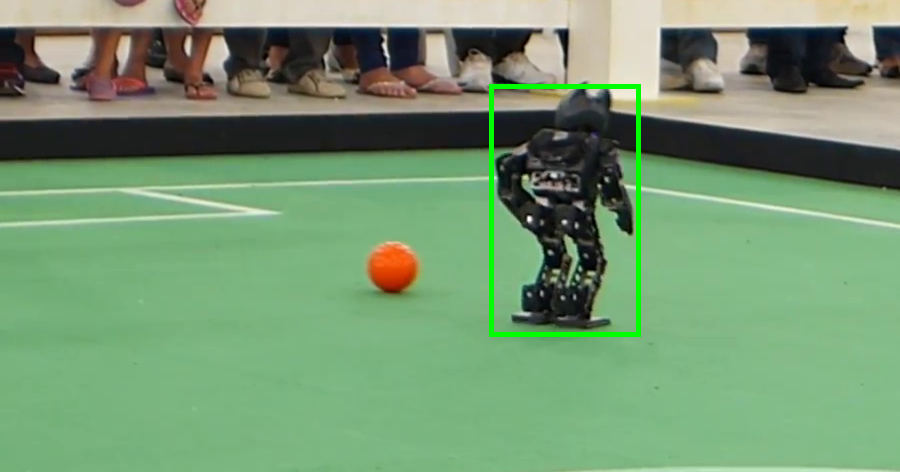
\includegraphics[width=8cm]{Imagens/HeartsHAAR.png}
\DeclareGraphicsExtensions.
\caption{Identificação do Robô Bold Hearts \cite{Bold} da universidade de Hertfordshire usando HAAR. \\ Fonte: Quadro extraído do video de qualificação do próprio time disponível no youtube.}
\label{fig_HeHAAR}
\end{figure}

\begin{figure}[!hH]
\centering
\includegraphics[width=8cm]{Imagens/HeartsHOG.png}
\DeclareGraphicsExtensions.
\caption{Identificação do Robô Bold Hearts \cite{Bold} da universidade de Hertfordshire usando HOG.\\ Fonte: Quadro extraído do video de qualificação do próprio time disponível no youtube.}
\label{fig_HeHOG}
\end{figure}


\section{Comparando os dois descritores e seus classificadores} 

O descritor HAAR teve um desempenho melhor que o descritor HOG em termos de velocidade, especialmente nas maiores resoluções. Entretanto quando o robô foi levado para o ambiente real, a iluminação se tornou um verdadeiro problema. Para ambos os algoritimos foi necessário incluir imagens negativas referentes ao ambiente. Na figura ~\ref{fig_rocHH} uma curva ROC que compara as capacidades e limitações dos dois algoritimos. 

\begin{figure}[!hH]
\centering
\includegraphics[width=12cm]{Imagens/ROCHH.png}\\
\DeclareGraphicsExtensions.
\caption{Curvas ROC. A linha verde mostra o algoritimo HOG-SVM clássico treinado com imagens de robôs usado para detecção de robôs.
A linha vermelha demonstra o resultado do classificador HAAR-AdaBoost treinado com o mesmo propósito.}
\label{fig_rocHH}
\end{figure}

As duas curvas ROC sugerem que os classificadores treinados parecem ser equivalentes. Devido à diversidade de robôs ambos os classificadores demonstraram capacidade de generalização que pode reconhecer diversos tipos de robôs dadas imagens de treinamento normalizadas suficientes.

Outro parâmetro de desempenho utilizado foi o de resposta dos algoritimos em quadros por segundo. É vital para um robô jogador de futebol que consiga detectar outros robôs em tempo real. A comparação desses parâmetros de desempenho estão na figura ~\ref{fig_fps}.

\begin{figure}[!hH]
\centering
\includegraphics[width=12cm]{Imagens/FPS.png}
\DeclareGraphicsExtensions.
\caption{Desempenho dos descritores HAAR-AdaBoost e HOG-SVM em termos de quadros por segundo após processamento. Esta informação é particularmente vital quando se trata de um robô que precisa agir rapidamente.\\ Fonte: O Autor}
\label{fig_fps}
\end{figure}

Os resultados mostram alguma vantagem para o HAAR-Adaboost em quadros por segundo, que pôde ser utlizado em full-hd 1920x1080 pixels mas, com alguns falso positivos, já que é uma técnica sensível à mudanças de iluminação. Já o HOG-SVM foi mais preciso em termos de detecção, porém com a limitação da taxa de velocidade e por consequência a resolução máxima de 640x480 pixels. Nas figuras ~\ref{fig:Mix1} e ~\ref{fig:Mix2} as mesmas imagens demonstrando as detecções para os dois algoritimos.

Aqui cabe uma ressalva, quando se trata de avaliar os descritores, os parâmetros escolhidos e o hardware foram verdadeiramente responsáveis pelo desempenho geral dos dois algoritimos.

O tempo gasto no treinamento e na normalização e redimensionamento das imagens tmabém foi uma questão complicada. Enquanto o HOG-SVM determinava todas as características por si só e levava no máximo 2 horas para efetuar o treinamento, o HAAR-Adaboost precisava que uma pessoa determinasse onde os objetos estavam em cada imagem positiva e seu treinamento levou de 5 a 12 horas para ser concluído. É válido lembrar que as imagens positivas do HOG-SVM precisaram ser redimensionadas o que levou um tempo considerável.


\begin{figure}[!hH]%
    \centering
    \subfloat[HOG - SVM]{{\includegraphics[width=10cm]{Imagens/MixHOG.png} }}%3.65
    \qquad
    \subfloat[HAAR - Boosting]{{\includegraphics[width=10cm]{Imagens/MixHAAR.png} }}%
    \caption{Vários robôs identificado usando o HOG-SVM e o HAAR-Boosting. Fonte: Quadro extraído do video de qualificação do time Bold Hearts - RoboCup 2015.}%
    \label{fig:Mix1}%
\end{figure}

\begin{figure}[!hH]%
    \centering
    \subfloat[HOG - SVM]{{\includegraphics[width=10cm]{Imagens/CIT01HOG.png} }}%3.65
    \qquad
    \subfloat[HAAR - Boosting]{{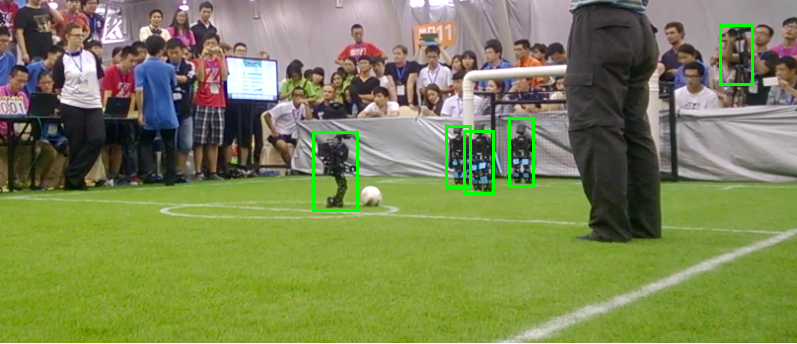
\includegraphics[width=10cm]{Imagens/CIT01HAAR.png} }}%
    \caption{Vários robôs identificado usando o HOG-SVM e o HAAR-Boosting. Fonte: O autor - RoboCup 2015.}%
    \label{fig:Mix2}%
\end{figure}

\pagebreak



\section{Experimento - Determinação da distância da bola ao robô}

Os cálculos das distâncias da bola e do robô até outros robôs, foram determinados de forma experimental, tabelando a distância em centímetros e a área dos objetos em pixels, encontrando uma função que representasse essa relação, considerando a resolução da captura. As funções experimentais obtidas, por meio de regressão, estão nos algoritmos propostos.


O principal objetivo da média móvel simples é fornecer o valor médio do raio da bola e sua posição em pixels dentro de um determinado período, no caso, os últimos 10 quadros da captura de video. Assim, para cada valor incluído no cálculo da média, o valor mais antigo é excluído. Na média móvel simples (SMA), cada dado utilizado no cálculo da média terá o mesmo peso. 

\begin{equation} 
	MRB = \frac {[R(q) + R(q-1) + R(q-2) + … + R(q-9)]}  {10}
\end{equation}\\

MRB é a média móvel do raio da bola e R é o raio da bola ambos em pixels, já "q" se refere ao indice do quadro atual da captura da camera. 

Tabelando os raios médios da bola e sua distância real em centímetros, é possível por meio de regressão estimar uma função que representa os dados. 30 pontos foram levantados com varições A bola foi posicionada à 50 centimetros do pé do robô, para cada incremento de 5 centimetros o raio médio da bola foi coletado, 

\begin{equation} 
	%D_{bola} = 3,7.10^{-7} * MRB^4 -7.9e^{-5} * MRB^3 +6.2e^{-3} * MRB^2 -2.2e^{-1} * MRB + 3.7 
	%D_{bola} = 331.59-53.3*log(MRB-50);
	D_{bola} = \frac {9143} {MRB}
\end{equation}\\

Essa função foi extraída para a resolução de 1920x1080 e bola de tamanho fixo conhecido de 13 centímetros, onde \(D_{\text{Bola}}\) é a distância da bola ao robô em centimetros, e MRB é a média móvel do raio da bola em pixels.

\begin{figure}[!t1]
\centering
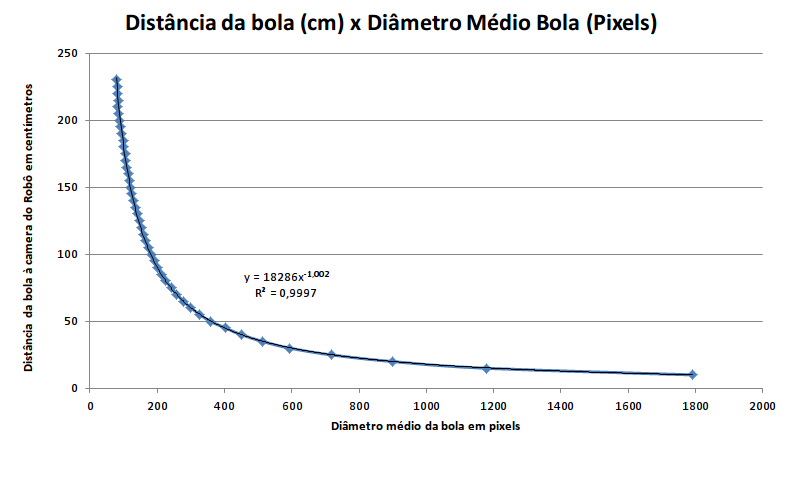
\includegraphics[width=10cm]{Imagens/Dist.png}
\DeclareGraphicsExtensions.
\caption{Função relacionando pixels com distância de uma bola de tamanho conhecido.}
\label{Fig:DistBall}
\end{figure}

É claro que, haverá um erro de medição nessas fórmulas, já que foram calculadas sem oclusão e com o objeto inteiro no campo de visão, nesse caso, o erro será proporcional à oclusão.


\section{Experimento - Determinação da distância do robô a outros robôs}

Para determinar as distâncias até os robôs adversários, ou até os companheiros de equipe é necessário que se possua todas as dimensões dos robôs da liga. Analisando os TDP's Artigos de descrição dos times de todos os robôs da liga KidSize, foram extraídos as alturas dos mesmos.
A tabela criada possui uma coluna referente ao número do time e uma ou mais colunas referente à altura do robôs de cada time, já que um time pode ter mais de um tipo de robô. 

Antes de se iniciar uma partida, o juiz procura os líderes de cada time para definição de suas respectivas cores. Duas cores são possíveis, o time vermelho tem uma coloração magenta e o time azul tem a cor ciano. Feita a escolha, os times devem revestir seus robôs com as cores definidas. A área mínima desses marcadores é 5x5 centímetros nos braços, pernas e tronco.

A abordagem experimental será abordada para esse caso, 

A detecção foi feita usando o descritor HAAR conforme parametros usados no capitulo ~\ref{HAAR-Boosting}

Somente dentro da janela de detecção do robô é feita uma segmentação da cor previamente escolhida no sistema HSV. Os valores foram discretizados em 20 valores para a matiz, 17 para a saturação e 17 para a intensidade.
Visto que para a resolução de 1920x1080 pixels a relação dis

Assim, se faz necessário encontrar uma fórmula que relacione a resolução da tela, o tamanho em pixels e o tamanho real do robô com a sua distância.

\pagebreak

%%===============================================================================


%*******************************************************************************************************
% 	Planejamento e Cronograma
%*******************************************************************************************************

\chapter{Conclusão}
\input{conclusion}

%%===============================================================================



\bibliography{Bibliografia}

\appendix
\chapter{Algoritmo de Detecção da Bola Laranja} 
\label{chap:apendiceBolaLaranja}
\section{Algoritmo de rastreamento da bola - Círculos de Hough.}

\begin{algorithm}

\Entrada{Abre Captura da Câmera (Dispositivo 0)}
\Se{Captura vazia}
	{Erro! Dispositivo não está pronto.
	Aborte Algoritmo.
		}

\Enqto{ Não for pressionada a tecla esc e Quadro não vazio}
{

Extraia um quadro RGB da captura, converta para uma imagem HSV.

\begin{equation}
     \centering
    	H = \left\{
		\begin{array}
		{ccl} 
		$$\theta, 	& Se B  \leq  G $$\\
		$$360 - \theta,	& Se B  >  G $$
		\end{array} 
\right.
\end{equation}

\begin{equation}
	\theta  =  \cos^-{^1} \left[  {   \frac {  \frac {1} {2} * [(R -G) + (R-B)]}  {  \sqrt{[(R -G)^2 + (R -B)(G -B)]}   }    }\right]
\end{equation}

\begin{equation}
	S  =  1 - { \frac {3} {(R+G+B)} } * [min (R,G,B)]
\end{equation}

\begin{equation}
	I  =  { \frac {1} {3}} * {(R+G+B)}
\end{equation}



\Entrada{Tabela de pesquisa (LUT). (0<H<35, 0<S<180, 0<V<255)}

\ParaTodo {Pixel dentro da imagem HSV e dentro dos limites da LUT}
	{Altere o valor do Pixel de uma matriz binária na mesma posição}

Na matriz binária aplique Erosão seguida da Dilatação. ( 5x5 Pixels)

Aplique filtro espacial. (Gaussiana 9x9 Pixels)

Transformada de Hough para círculos:

- Atualize a média móvel do raio (MRB) e da posição XY dos círculos encontrados.

\begin{equation} 
	D_{bola} = \frac {9143} {MRB}
\end{equation}\\

Armazene \(D_{bola}\), a posição dos servos Pan-Tilt em graus e da bola em pixels.
}

\Retorna \(D_{bola}\)

\caption[Algoritmo de rastreamento da bola - Círculos de Hough.]{Fonte: Autor.}
\label{lst:algBall}
\end{algorithm}


\chapter{Algoritmo para divisão do Quadro} \label{chap:apendiceDivQuadro}

\section{Algoritmo para buscar e centralizar o objeto.}
\begin{algorithm}

Divida o quadro de captura em 3 regiões horizontais, sendo a região central com 5\% da resolução horizontal.\\
Divida o quadro de captura em 3 regiões verticais, sendo a região central com 5\% da resolução vertical.\\
\Enqto{Quadro não vazio}
{
	\Se{Dentro do quadro houver objeto}
		{
		Encontre em qual região o objeto se encontra usando sua posição.\\
				\Se {O objeto estiver na região 5 (central)} 
					{Mantenha o objeto nessa região parando o movimento}
				\Se {O objeto estiver nas regiões 1, 4 e 7} 
					{Some a posição atual do servo com a quantidade de graus para o pan}
				\Se {O objeto estiver nas regiões 3, 6 e 9} 
					{Subtraia a posição atual do servo com a quantidade de graus para o pan}
				\Se {O objeto estiver nas regiões 1, 2 e 3} 
					{Some a posição atual do servo com a quantidade de graus para o tilt}
				\Se {O objeto estiver nas regiões 7, 8 e 9} 
					{Subtraia a posição atual do servo com a quantidade de graus para o tilt}
		Guarde posição dos servos\\
		}
		\Senao
		{		
		Chame algoritmo de busca \ varredura
		}
	
}
\Retorna \(Posicao do Servo\)

\caption[Algoritmo para buscar e centralizar o objeto]{Fonte: Autor}
\label{lst:algCent}
\end{algorithm}



\chapter{Algoritmo para Identificação de Robôs. (HOG-SVM)} \label{chap:apendiceHOG}

\section{HOG-SVM Offline}
\begin{algorithm}


\Entrada{Conjunto de imagens positivas - Contém robôs participantes}
\Entrada{Conjunto de imagens negativas - Não contém robôs}

Extraia, do diretório de imagens negativas, todas as imagens que possuam tamanho e extensão compatíveis (jpg,jpeg,png,bmp)

Calcule o histograma de gradientes para todas as imagens.

Armazene o vetor de características (descritores) de cada uma das imagens negativas.

Extraia, do diretório de imagens positivas, todas as imagens que possuam tamanho e extensão compatíveis (jpg,jpeg,png,bmp)

Calcule o histograma de gradientes para todas as imagens desse diretório.

Armazene o vetor de características (descritores) de cada uma das imagens positivas.

Armazene o vetor de características (descritores) de cada uma das imagens negativas.

\Entrada{Vetores de características (descritores) das imagens positivas}
\Entrada{Vetores de características (descritores) das imagens negativas}

Determine os vetores de suporte e o hiperplano que melhor separa as duas classes usando o SVM.

\Entrada{Tabela com todas as alturas de todos os robôs de todos os times}
\Entrada{Tabela com a cor do time adversário}

\label{lst:algROF}
\caption[Algoritmo para Identificação de Robôs. (HOG-SVM Offline)]{Fonte: Autor.}
\end{algorithm}

\pagebreak

\section{HOG-SVM Online}

\begin{algorithm}


\Entrada{Hiperplano proveniente do SVM}
\Entrada{Aquisição da câmera}

\Enqto{ Quadro não vazio}
{
Calcule o histograma de gradientes da imagem adquirida da câmera

Extraia o vetor de caracterísiticas (descritores) da imagem adquirida.

Use o SVM para classificar o vetor de caracterísiticas da imagem adquirida.

	\Se {Houver robô presente na imagem}
	{
		Para cada bloco da imagem adquirida, encontre em qual bloco do histograma normalizado o robô se encontra\\

		Calcule sua altura em pixels\\

		Armazene o centro do bloco e a altura em pixels\\

		Segmentação da cor do time.\\

		Se a área na qual o robô for identificado conter o centroide referente à cor do time\\

		Busque na tabela de alturas qual a altura em centímetros do robô que foi identificado\\

		Calcule sua distância real até o robô em centímetros\\
	}

}
\caption[Algoritmo para Identificação de Robôs. (HOG-SVM Online)]{Fonte: Autor.}
\label{lst:algROn}
\end{algorithm}


\chapter{Algoritmo para Identificação de Robôs. (HAAR-Adaboost)} \label{chap:apendiceHAAR}

\section{HAAR-Adaboost Offline}
\begin{algorithm}

\Entrada{Conjunto de imagens positivas - Contém robôs participantes}
\Entrada{Conjunto de imagens negativas - Não contém robôs}

\Entrada{Posição dos robôs contidos nas imagens positivas}

\ParaTodo {Estágio da árvore e para todas as imagens}
{
\Enqto{\(Min_{\text{TaxaAcerto}}\) = 0,999 não atingida}
	{
	Extraia as características de HAAR para as imagens positivas.\\
	Execute o Adaboost conforme algoritmo ~\ref{lst:algHaar} usando como parâmetros:\\
		- Tamanho da amostra = 20x20 Pixels;\\
		- Tamanho mínimo do objeto = 30x30 Pixels;\\
		- Tamanho máximo do objeto = Resolução vertical x \( \frac {Resolução Horizontal}{2}\) Pixels\\
		- Classificador 8 Vizinhos mais próximos. \\
	}
	Armazene a hipótese final do estágio.\\
}
	Armazene a hipótese final em um arquivo .xml

\caption[Algoritmo de Identificação de robôs. (HAAR-Adaboost Offline)]{Fonte: Autor ``Adaptado de'' \citefloat{Adaboost} }
\label{lst:algHaarOF}
\end{algorithm}

\pagebreak

\section{HAAR-Adaboost Online}
\begin{algorithm}

\Entrada{Árvore proveniente do Adaboost (Arquivo .xml)}

\Entrada{Aquisição da câmera}

\Enqto{ Quadro não vazio}
{

Extraia o vetor de caracterísiticas (descritores) da imagem adquirida.\\
Percorra os nós (Estágios) da árvore presentes no arquivo xml encontrando a melhor classificação para a imagem adquirida\\

	\Se {Houver robô presente na imagem}
	{
		Para cada bloco da imagem adquirida, encontre em qual bloco o robô se encontra\\

		Calcule sua altura em pixels\\

		Armazene o centro do bloco e a altura em pixels\\

		Segmentação da cor do time.\\

		Se a área na qual o robô for identificado conter o centroide referente à cor do time\\

		Busque na tabela de alturas qual a altura em centímetros do robô que foi identificado\\

		Calcule sua distância real até o robô em centímetros\\
	}
}

\caption[Algoritmo de Identificação de robôs. (HAAR-Adaboost Online)]{Fonte: Autor ``Adaptado de''\citefloat{Adaboost} }
\label{lst:algHaarOn}
\end{algorithm}


	

%\indice

\end{document}
